%<dscrpt>Intégrale curviligne et géométrie sphérique.</dscrpt>
L'objet de ce problème est l'étude d'une certaine intégale curviligne le long d'une portion d'ellipse qui est obtenue par projection d'un demi grand cercle tracé sur la sphère unité.\newline
On se place dans un espace affine euclidien muni d'un repère orthonormé $\mathcal{R}=(O,\mathcal{B})$ avec $\mathcal{B}=(\overrightarrow{i},\overrightarrow{j},\overrightarrow{k})$. On note $\mathcal{S}$ la demi-sphère unité formée par les points dont les coordonnées $(x,y,z)$ vérifient $x^2+y^2+z^2=1$ avec $z > 0$.\newline
Dans tout le problème $\varphi$ appartient à $]0,\frac{\pi}{2}[$.
\begin{figure}[h!t]
 \centering
 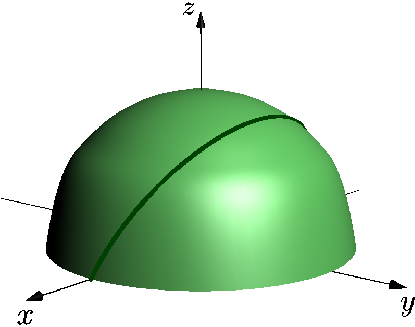
\includegraphics{./Eintcurv_1.pdf}
 % Eintcurv_1.pdf: 0x0 pixel, -2147483648dpi, 0.00x0.00 cm, bb=
 \caption{Un demi grand cercle sur la shpère unité.}
 \label{fig:Eintcurv_1}
\end{figure}
\subsection*{Partie I. Projection d'un demi grand cercle}
\begin{figure}[h!t]
 \centering
 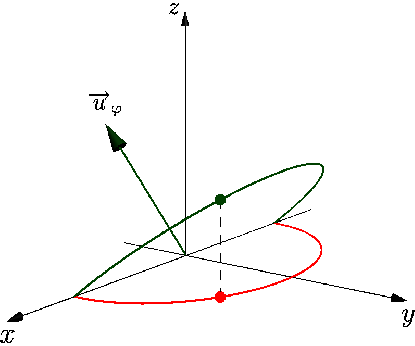
\includegraphics{./Eintcurv_2.pdf}
 % Eintcurv_1.pdf: 0x0 pixel, -2147483648dpi, 0.00x0.00 cm, bb=
 \caption{Projection d'un demi grand cercle.}
 \label{fig:Eintcurv_2}
\end{figure}
Soit $\overrightarrow{u}_\varphi$ le vecteur de coordonnées $(0,-\sin \varphi, \cos \varphi)$ dans $\mathcal{B}$. On note $\mathcal{C}_\varphi$ l'intersection du plan orthogonal à $\overrightarrow{u}_\varphi$ passant par $O$ et de $\mathcal{S}$. On note $\mathcal{E}_\varphi$ la projection orthogonale de $\mathcal{C}_\varphi$ sur le plan $(O,\overrightarrow{i},\overrightarrow{j})$.
\begin{enumerate}
 \item
\begin{enumerate}
\item Soit $M$ un point du plan $(O,\overrightarrow{i},\overrightarrow{j})$ de coordonnées $(x,y)$. Sous quelle condition portant sur $x$ et $y$ le point $M$ est-il dans $\mathcal{E}_\varphi$?
\item En déduire que $\mathcal{E}_\varphi$ est une conique dont on précisera le genre, l'axe focal et les foyers.
\end{enumerate}
\item Soit $\mathcal{B}_\varphi$ une base orthonormée directe $(\overrightarrow{i},\overrightarrow{j}_\varphi,\overrightarrow{u}_\varphi)$ et $\theta$ un nombre réel.
\begin{enumerate}
 \item Former la matrice dans $\mathcal{B}_\varphi$ de la rotation d'angle $\theta$ autour de $\overrightarrow{u}_\varphi$. On note $r_{\theta,\varphi}$ cette rotation.
 \item Calculer les coordonnées de $\overrightarrow{j}_\varphi$ dans $\mathcal{B}$ puis la matrice de $r_{\theta,\varphi}$ dans $\mathcal{B}$.
 \item On note $M_\theta$ le point $O+r_{\theta,\varphi}(\overrightarrow{i})$. Pour quels $\theta$ le point $M_\theta$ est-il dans $\mathcal{C}_\varphi$ ? En déduire une paramétrisation de $\mathcal{E}_\varphi$
\begin{displaymath}
 \theta \rightarrow P_\theta
\end{displaymath}
\end{enumerate}

\end{enumerate}
\subsection*{Partie II. Intégrale curviligne.}
\begin{figure}[h!t]
 \centering
 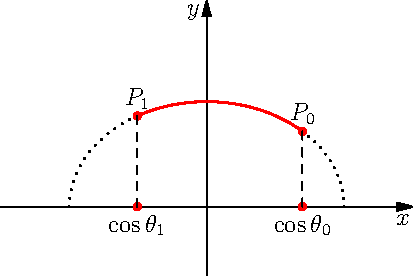
\includegraphics{./Eintcurv_3.pdf}
 \caption{Arc d'ellipse}
 \label{fig:Eintcurv_3}
\end{figure}
Dans cette partie, $x$ et $y$ désignent les fonctions coordonnées associées au repère $(O,\overrightarrow{i},\overrightarrow{j})$ dans le plan $(O,\overrightarrow{i},\overrightarrow{j})$.\newline
On considère la forme différentielle $\omega$ définie dans la plan (privé de $O$) par
\begin{displaymath}
 \omega = \frac{\sqrt{1-x^2-y^2}}{3(x^2+y^2)}\left(y\,dx - x\,dy \right) 
\end{displaymath}
On considère la demi ellipse d'équation
\begin{displaymath}
 x^2 + \frac{1}{\cos^2 \varphi}y^2 = 1 \hspace{1cm} y > 0
\end{displaymath}
On note $\Gamma$ l'arc orienté sur cette demi ellipse de $P_0$ à $P_1$ respectivement de coordonnées $\cos \theta_0$ et $\cos \theta_1$ avec $\theta_0>0$ et $\theta_1>0$.
\begin{enumerate}
 \item Calculer l'intégrale
\begin{displaymath}
 \int_{\theta_0}^{\theta_1}\frac{\sin \theta}{\cos^2 \varphi +\sin^2\varphi \cos^2\theta}d\theta
\end{displaymath}
\item Calculer l'intégrale curviligne de $\omega$ le long de $\Gamma$.
\end{enumerate}

\subsection*{Partie III. Expression vectorielle.}
\begin{figure}[h!t]
 \centering
 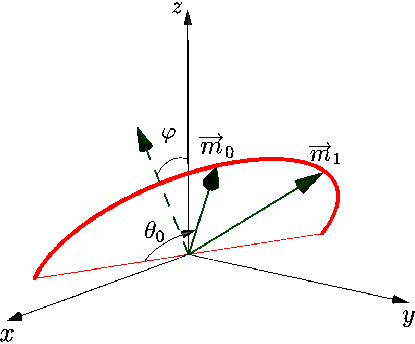
\includegraphics{./Eintcurv_4.pdf}
 \caption{Deux vecteurs dans la demi sphère}
 \label{fig:Eintcurv_4}
\end{figure}
On se donne deux vecteurs unitaires $\overrightarrow{m}_0$ et $\overrightarrow{m}_1$ respectivement de coordonnées $(a_0,b_0,c_0)$ et $(a_1,b_1,c_1)$ tels que $c_0>0$ et $c_1>0$.\newline
Soit $\overrightarrow{u}$ le vecteur unitaire orthogonal à $\overrightarrow{m}_0$ et $\overrightarrow{m}_1$ dont le produit scalaire avec $\overrightarrow{k}$ est strictement positif et $\varphi$ l'écart angulaire entre $\overrightarrow{k}$ et $\overrightarrow{u}$.\newline
Soit $\overrightarrow{I}$ le vecteur unitaire orthogonal à $\overrightarrow{u}$ et $\overrightarrow{k}$ tel que $(\overrightarrow{k},\overrightarrow{u},\overrightarrow{I})$ soit directe.\newline
Soit $\overrightarrow{J}$ le vecteur unitaire tel que $(\overrightarrow{I},\overrightarrow{J},\overrightarrow{k})$ soit une base orthonormée directe.
\begin{enumerate}
 \item 
\begin{enumerate}
 \item  Montrer qu'il existe $\varepsilon \in\{-1,+1\}$ tel que 
\begin{displaymath}
 \overrightarrow{u} = 
\frac{\varepsilon}{\left\Vert\overrightarrow{m_0}\wedge \overrightarrow{m_1}\right\Vert}\,\overrightarrow{m_0}\wedge \overrightarrow{m_1}
\end{displaymath}
 \item Exprimer $\cos \varphi$ et $\sin \varphi$ à l'aide de produits vectoriels et scalaire. En déduire que $\varphi \in ]0,\frac{\pi}{2}[$.
\end{enumerate}

 \item Montrer qu'il existe un réel $\lambda >0$ tel que  $\overrightarrow{J} = -\varepsilon\lambda p(\overrightarrow{m_0}\wedge \overrightarrow{m_1})$ où $p$ désigne la projection orthogonale sur $\Vect(\overrightarrow{i},\overrightarrow{j})$.
 
 \item \begin{enumerate}
 \item Montrer que 
\begin{displaymath}
 (\overrightarrow{J}/\overrightarrow{m_0}) =
\varepsilon \lambda \,(\overrightarrow{m_0}\wedge \overrightarrow{m_1}/\overrightarrow{k})\,
(\overrightarrow{m_0}/ \overrightarrow{k})  
\end{displaymath}

 \item Montrer qu'il existe des réels $\theta_0$ et $\theta_1$ dans $]0,\pi[$ tels que 
\begin{displaymath}
 \overrightarrow{m}_0 = r_{\theta_0,\overrightarrow{u}}(\overrightarrow{I})
\hspace{1cm}
\overrightarrow{m}_1 = r_{\theta_1,\overrightarrow{u}}(\overrightarrow{I})
\end{displaymath}
(la notation $r_{\theta,\overrightarrow{u}}$ désigne la rotation d'angle $\theta$ autour de $\overrightarrow{u}$) 
\end{enumerate}
\item En exprimant $\cos \theta_0$ et $\cos \varphi$ en fonction de $\varepsilon$, $\sin(\theta_1-\theta_0)$, $\sin \varphi$ et de produits scalaires et vectoriels, montrer que
\begin{displaymath}
 \cos \theta_0 \tan \varphi = 
\frac{(\overrightarrow{m_0}\wedge \overrightarrow{k}/\overrightarrow{m_0}\wedge \overrightarrow{m_1})}
{(\overrightarrow{k}/\overrightarrow{m_0}\wedge \overrightarrow{m_1})}
\end{displaymath}

\end{enumerate}